%%%%%%%%%%%%%%%%%%%%%%%%%%%%%%%%%%%%%%%%%%%%%%%%%%%%%%%%%%%%%%%%%%%%%%%%%%%%%%%%%%%
%%%%%%%%%%%
%%%%%%%%%%% DIMENSION UUMUS example
\begin{figure}
\centering

\ifx\USETIKZINFIGURE\undefined
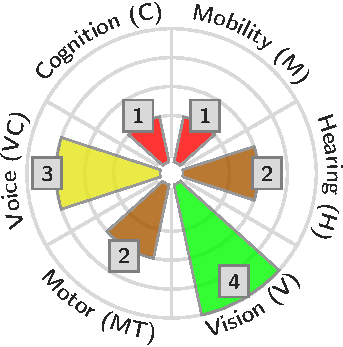
\includegraphics{figures/jVRARVestfold-UUMUS}
\else
\begin{tikzpicture}[scale=0.70]

\renewcommand{\UUMUSfontsize}{\small}
\renewcommand{\UUMUSareafontsize}{\small}
\renewcommand{\UUMUSnumberfontsize}{\small}
%\renewcommand{\UUMUSlabeladjustment}{-0.5mm}
%\renewcommand{\UUMUSraise}{-1.0ex}
\renewcommand{\UUMUSraise}{-0.5ex}

\path (\UUMUSL+\UUMUSLXX+2mm,\UUMUSL+\UUMUSLXX+2.5mm) --
(-\UUMUSL-\UUMUSLXX-2mm,\UUMUSL+\UUMUSLXX+2.5mm) --
(-\UUMUSL-\UUMUSLXX-2mm,-\UUMUSL-\UUMUSLXX-2.5mm) --
(\UUMUSL+\UUMUSLXX+2mm,-\UUMUSL-\UUMUSLXX-2.5mm);

% Draw background
\UUMUSdraw
% Draw labels
\UUMUStext{xxx}{1}{Cognition (C)}
\UUMUStext{xxx}{2}{Voice (VC)}
\UUMUStext{xxx}{3}{Motor (MT)}
\UUMUStext{xxx}{4}{Vision (V)}
\UUMUStext{xxx}{5}{Hearing (H)}
\UUMUStext{xxx}{6}{Mobility (M)}

% Draw in sector 1
\foreach \X in {1,2,...,6}{%
%\UUMUSdrawfill{fill=black}{\X}{0}
%\UUMUSdrawfill{fill=black!25!white}{\X}{3}
}

%\UUMUSfillborder{color=black!40!white, opacity=0.5}{1}{3}{3} % 0-ring
%\UUMUSfillarea{pattern=north east lines, pattern color=brown!60!black}{1}{2}{3} 
%\UUMUSline{color=orange,line width=2pt}{1}{3}
%\UUMUSdrawfill{fill=white!40!blue}{1}{0} % 

% Draw in sector 1C
%\UUMUSfillareanarrow{color=red!99!green, opacity=0.9}{1}{0}{1} 
\UUMUSuumus{1}{1}
%\UUMUSlabelbox{1}{1}{1}

% Draw in sector 2S
%\UUMUSfillareanarrow{color=red!66!green, opacity=0.9}{2}{0}{2} 
\UUMUSuumus{2}{3}

% Draw in sector 3M
%\UUMUSfillareanarrow{color=yellow!66!green, opacity=0.9}{3}{0}{3} 
\UUMUSuumus{3}{2}

% Draw in sector 4V
%\UUMUSfillareanarrow{color=red!1!green, opacity=0.9}{4}{0}{4} 
\UUMUSuumus{4}{4}

% Draw in sector 5H
%\UUMUSfillareanarrow{color=red!99!green, opacity=0.9}{5}{0}{1} 
\UUMUSuumus{5}{2}

% Draw in sector 6M
%\UUMUSfillareanarrow{color=red!99!green, opacity=0.9}{6}{0}{1} 
\UUMUSuumus{6}{1}


% colour formula: (value - 40) * 4
%\node at (0,{\UUMUSR/\UUMUSU*(1+1.4)}) {\mytextstyle -\,-}; 
%\node at (0,{\UUMUSR/\UUMUSU*(2+1.4)}) {\mytextstyle -}; 
%\node at (0,{\UUMUSR/\UUMUSU*(3+1.4)}) {\mytextstyle 0}; 
%\node at (0,{\UUMUSR/\UUMUSU*(4+1.4)}) {\mytextstyle +}; 
%\node at (0,{\UUMUSR/\UUMUSU*(5+1.4)}) {\mytextstyle ++}; 

\renewcommand{\UUMUSfontsize}{\scriptsize} % set to original value
\end{tikzpicture}
%
\fi
%
\caption{Eksempel UUMUS}
\label{fig:UUMUS:kunst}
\end{figure}
%%%%%%%%%%%%%%%%%%%%%%%%%%%%%%%%%%%%%%%%%%%%%%%%%%%%%%%%%%%%%%%%%%%%%%%%%%%%%%%%
%%%%%%%%%%%%%%%%%%%%%%%%%%%%%%%%%%%%%%%%%%%%%%%%%%%%%%%%%%%%%%%%%%%%%%%%%%%%%%%%
